\documentclass[aspectratio=169,10pt]{beamer}
\usetheme[
%%% options passed to the outer theme
%    progressstyle=movCircCnt,   %either fixedCircCnt, movCircCnt, or corner
%    rotationcw,          % change the rotation direction from counter-clockwise to clockwise
%    shownavsym          % show the navigation symbols
  ]{AAUsimple}
  
% If you want to change the colors of the various elements in the theme, edit and uncomment the following lines
% Change the bar and sidebar colors:
%\setbeamercolor{AAUsimple}{fg=red!20,bg=red}
%\setbeamercolor{sidebar}{bg=red!20}
% Change the color of the structural elements:
%\setbeamercolor{structure}{fg=red}
% Change the frame title text color:
%\setbeamercolor{frametitle}{fg=blue}
% Change the normal text color background:
%\setbeamercolor{normal text}{fg=black,bg=gray!10}
% ... and you can of course change a lot more - see the beamer user manual.

\usepackage[utf8]{inputenc}
\usepackage[danish]{babel}
\usepackage[T1]{fontenc}
% Or whatever. Note that the encoding and the font should match. If T1
% does not look nice, try deleting the line with the fontenc.
\usepackage{helvet}
\usepackage{booktabs}
\renewcommand{\arraystretch}{1.5}
\usepackage{tikz}
\usepackage{pgfplots}
\newcommand{\boundellipse}[3]% center, xdim, ydim
{(#1) ellipse (#2 and #3)
}
\tikzset{
	invisible/.style={opacity=0},
	visible on/.style={alt={#1{}{invisible}}},
	alt/.code args={<#1>#2#3}{%
		\alt<#1>{\pgfkeysalso{#2}}{\pgfkeysalso{#3}} % \pgfkeysalso doesn't change the path
	},
}
% colored hyperlinks
\newcommand{\chref}[2]{%
  \href{#1}{{\usebeamercolor[bg]{AAUsimple}#2}}%
}
\setbeamercovered{transparent} 
%
%
%% Macros
%
%
%
\newcommand{\R}{\mathbb{R}}


\title{Math101}

% \subtitle{}  % could also be a conference name

\date{\today}

\author{
  Benjamin Støttrup\\
  \href{mailto:benjamin@math.aau.dk}{{\tt benjamin@math.aau.dk}}
}

% - Give the names in the same order as they appear in the paper.
% - Use the \inst{?} command only if the authors have different
%   affiliation. See the beamer manual for an example

\institute[
%  {\includegraphics[scale=0.2]{aau_segl}}\\ %insert a company, department or university logo
  Institut for matematiske fag\\
  Aalborg universitet\\
  Danmark
] % optional - is placed in the bottom of the sidebar on every slide
{% is placed on the bottom of the title page
  Institut for matematiske fag\\
  Aalborg universitet\\
  Danmark
  
  %there must be an empty line above this line - otherwise some unwanted space is added between the university and the country (I do not know why;( )
}

% specify a logo on the titlepage (you can specify additional logos an include them in 
% institute command below
\pgfdeclareimage[height=1.5cm]{titlepagelogo}{AAUgraphics/aau_logo_new} % placed on the title page
%\pgfdeclareimage[height=1.5cm]{titlepagelogo2}{AAUgraphics/aau_logo_new} % placed on the title page
\titlegraphic{% is placed on the bottom of the title page
  \pgfuseimage{titlepagelogo}
%  \hspace{1cm}\pgfuseimage{titlepagelogo2}
}
%\includeonly{sections/slides5}
\begin{document}
% the titlepage
{\aauwavesbg%
\begin{frame}[plain,noframenumbering] % the plain option removes the header from the title page
  \titlepage
\end{frame}}
%%%%%%%%%%%%%%%%

% TOC
\begin{frame}{Agenda}{}
\tableofcontents
\end{frame}
%%%%%%%%%%%%%%%% 
%\section{Brøker}
\begin{frame}{Brøker}
\begin{itemize}
		\setlength\itemsep{1em}
	\item<1-> \emph{Brøker} er tal på formen
	\begin{align*}
	\frac{a}{b},
	\end{align*}
	hvor $a$ og $b$ er reelle tal og $b\neq 0$.
	\item<2->  Vi kalder $a$ for brøkens \emph{tæller} og $b$ for brøkens \emph{nævner}.
	\item<3-> En brøk $\frac{a}{b}$ skal forstås som $a$ divideret med $b$.
	\item<4-> Vi vil kun tænke på $\frac{a}{b}$ som decimaltal hvis $b$ går op i $a$.
	
	Eksempelvis er $\frac{1}{3}\neq 0.33$.
\end{itemize}

\end{frame}
\begin{frame}{Brøker}{Regneregler}
\begin{itemize}
		\setlength\itemsep{1em}
	\item<1-> For brøker har vi følgende regneregler
	\begin{align*}
	\onslide<1->{\frac{a}{c}\pm\frac{b}{c}=\frac{a\pm b}{c},}&&\onslide<2->{\frac{a}{b}\frac{c}{d}=\frac{ac}{bd},}&&\onslide<3->{\frac{\frac{a}{b}}{\frac{c}{d}}=\frac{ad}{bc},}\\
	\onslide<4->{a\frac{b}{c}=\frac{ab}{c},}&& \onslide<5->{\frac{\frac{a}{b}}{c}=\frac{a}{bc},}&&\onslide<6->{\frac{a}{\frac{b}{c}}=\frac{ac}{b}.}
	\end{align*}
	\item<7-> Eksempler: Udregn
\end{itemize}
	\begin{align*}
\onslide<7->{\frac{4}{5}-\frac{2}{5},}&&\onslide<8->{\frac{3}{4}\cdot\frac{9}{4},}&&\onslide<9->{\frac{\frac{1}{2}}{\frac{3}{5}},}\\
\onslide<10->{2\cdot\frac{4}{5},}&& \onslide<11->{\frac{\frac{4}{3}}{7},}&&\onslide<12->{\frac{5}{\frac{2}{3}}.}
\end{align*}
\end{frame}

\begin{frame}{Brøker}{Forkorte/Forlænge}
\begin{itemize}
		\setlength\itemsep{1em}
	\item<1-> Man kan gange (dividere) en brøks tæller og nævner med samme tal (bortset fra 0) uden at ændre værdien af brøken:
	\begin{align*}
	\frac{a}{b}=\frac{a}{b}\cdot1=\frac{a}{b}\cdot \frac{c}{c}=\frac{ac}{bc}.
	\end{align*}
	\item<2-> Dette kaldes at forlænge (forkorte) en brøk. 
	\item<3-> Vi vil altid forkorte et svar på en opgave så meget som muligt.
	\item<4-> Eksempler: Udregn
	\begin{align*}
	\frac{1}{2}+\frac{3}{4},&& \onslide<5->{\frac{6}{8}\cdot\frac{1}{4}}
	\end{align*}
	\item<6-> Eksempel: Reducer udtrykket
	\begin{align*}
	\frac{ab+a^2b}{a(1+a)}.
	\end{align*}
\end{itemize}
\end{frame}



\section{Potenser}
\begin{frame}{Potenser}
\begin{itemize}
		\setlength\itemsep{1em}
	\item<1-> Hvis vi ganger et tal $x$ med sig selv $n> 0$ gange kaldes det resulterende tal for $x^n$. Altså
	\begin{align*}
	x^n=\underbrace{x \cdot x \cdot \dots \cdot x}_{\textup{n gange}}.
	\end{align*}
	\item<2-> $x$ kaldes grundtallet og $n$ kaldes eksponenten.
	\item<3-> Hvis $n<0$ så er
	\begin{align*}
	x^n=\frac{1}{x^{-n}}=\frac{1}{\underbrace{x \cdot x \cdot \dots \cdot x}_{\textup{n gange}}}.
	\end{align*}
	\item<4-> Specielt gælder at $x^0=1$ og at $0^0$ ikke defineres.
	\item<5-> Eksempler: Udregn $3^4$, $2^{-3}$ og $0^8$.
\end{itemize}
\end{frame}

\begin{frame}{Potenser}{Regneregler}
\begin{itemize}
		\setlength\itemsep{1em}
	\item<1-> For potenser har vi følgende regneregler
	\begin{align*}
	\onslide<1->{x^ax^b=x^{a+b},}&& \onslide<2->{\frac{x^a}{x^b}=x^{a-b},}&&\onslide<3->{(xy)^a=x^ay^a,}\\
	\onslide<4->{\Big(\frac{x}{y}\Big)^a=\frac{x^a}{y^a},}&&\onslide<5->{(x^a)^b=x^{ab},}&& \onslide<6->{x^{-a}=\frac{1}{x^a}.}	\end{align*}
	\item<7-> Bemærk at vi ikke har præsenteret nogle regneregler for potenser på formen $(x+y)^a$
	\item<8-> Eksempler: Udregn følgende
\end{itemize}
\begin{align*}
\onslide<8->{\frac{(2\cdot3)^2}{2^3},}&& \onslide<9->{\Big(\frac{2^3}{3}\Big)^{-2},}&& \onslide<10->{(-x)^2-x^2.}
\end{align*}
\end{frame}


\section{Rødder}
\begin{frame}{Rødder}
\begin{itemize}
		\setlength\itemsep{1em}
	\item<1-> For ethvert $x\geq 0$ og ethvert positivt heltal $n$ findes der et tal $\sqrt[n]{x}\geq 0$ så
	\begin{align*}
	(\sqrt[n]{x})^n=x.
	\end{align*}
%	\item Bemærk, at $(x^{\frac{1}{n}})^n=x^{\frac{n}{n}}=x.$
%	Dermed er $x^{\frac{1}{n}}=\sqrt[n]{x}$.% hvilket viser at rødder er potenser med eksponent $\frac{1}{n}$.	
	\item<2-> Hvis $n$ er lige så er $(\pm \sqrt[n]{x})^n=x$. Eksempelvis er $(-2)^2=2^2$.
	\item<3-> Hvis $n$ er ulige kan man godt tage en $n$'te rod af et negativt tal. Eksempelvis er $\sqrt[3]{-8}=-2$.
%	\item Hvis $n=2$ skriver vi $\sqrt{x}$ i stedet for $\sqrt[2]{x}$.
	\item<4-> Eksempler: Udregn $\sqrt{81}$,  $\sqrt[4]{16}$ og $\sqrt[n]{x^n}$.
\end{itemize}
\end{frame}
\begin{frame}{Rødder}{Regneregler}
\begin{itemize}
		\setlength\itemsep{1em}
	\item<1-> For rødder har vi følgende regneregler
	\begin{align*}
	\onslide<1->{\sqrt[n]{x}=x^{\frac{1}{n}},}&&\onslide<2->{ \sqrt[n]{x^m}=x^{\frac{m}{n}}=(\sqrt[n]{x})^m,}&&\onslide<3->{\sqrt[n]{xy}=\sqrt[n]{x}\sqrt[n]{y},}&& \onslide<4->{\sqrt[n]{\frac{x}{y}}=\frac{\sqrt[n]{x}}{\sqrt[n]{y}}.}
	\end{align*}
	\item<5-> Bemærk, at vi har mange regneregler som er ``ens'' for rødder og potenser.
	\item<6-> Eksempler: Udregn

\end{itemize}
\begin{align*}
\onslide<6->{\sqrt[3]{5^6},}&&\onslide<7->{ \sqrt{\sqrt{\sqrt{256}}},}&&\onslide<8->{\sqrt{\frac{144}{81}},}&&\onslide<9->{ \frac{3}{\sqrt{3}},}&& \onslide<10->{\frac{\sqrt{27}}{3}.}
\end{align*}
\end{frame}

\section{Kvadratsætninger}
\begin{frame}{Kvadratsætninger}
\begin{itemize}
		\setlength\itemsep{1em}
	\item<1-> Vi har set at $(xy)^n=x^ny^n$. Vi vil nu se at udtrykket $(x+y)^n$ ikke er helt så let at håndtere. 
	\item<2-> Vi har følgende formler
	\begin{align*}
	(a+b)^2&=a^2+b^2+2ab\\
	(a-b)^2&=a^2+b^2-2ab\\
	(a+b)(a-b)&=a^2-b^2.
	\end{align*}
	\item<3-> Eksempler: Reducer
\end{itemize}
\begin{align*}
\onslide<3->{(x+y)^2+(x-y)^2-x^2-y^2,}&&\onslide<4->{ \frac{1}{a+b}+\frac{1}{a-b},}&&\onslide<5->{\frac{2x^2+2-4x}{2x^2-2}.}
\end{align*}
\end{frame}


%\section{Førstegradsligninger}
\begin{frame}{Førstegradslignigner}
\begin{itemize}
		\setlength\itemsep{1em}
	\item<1-> En ligning består af to udtryk adskilt af et lighedstegn, hvor mindst et af udtrykkene indeholder en ubekendt variabel.
	\item<2-> En ligning løses ved at bestemme alle tal der kan indsættes på variablens plads så ligningen er sand.
	\item<3-> Eksempler:
\end{itemize}
	\begin{align*}
\onslide<3->{x+2=7,}&& \onslide<4->{2(x-1)=2x+3,}\\ \onslide<5->{x^2=9,}&&\onslide<6->{ x+1=\frac{1}{2}(2x+2).}
\end{align*}
\end{frame}

\begin{frame}{Førstegradsligninger}
\begin{itemize}
		\setlength\itemsep{1em}
	%\item For komplicerede ligninger kan vi ikke bare aflæse løsningerne.
	\item<1-> Ligninger kan reduceres med følgende regler:
	\begin{itemize}
			\setlength\itemsep{1em}
		\item<2-> Man må lægge til og trække fra med det samme tal på begge sider af et lighedstegn.
		\item<3-> Man må gange og dividere med det samme tal (undtagen 0) på begge sider af et lighedstegn.
	\end{itemize}
%	\item Strategi: Saml alle led som indeholder den ubekendte på den ene side af lighedstegnet og alle andre led på den modsatte side af lighedstegnet.
	\item<4-> Eksempler: Løs ligningerne

\end{itemize}
	\begin{align*}
\onslide<4->{4x+7=3(x+8),}&& \onslide<5->{\frac{2x+1}{4x}=3,}&& \onslide<6->{\pi x=3-2x.}
\end{align*}
\end{frame}

\section{Andengradsligninger}
\begin{frame}{Andengradsligninger}
\begin{itemize}
		\setlength\itemsep{1em}
	\item<1-> Vi betragter andengradsligninger på formen
	\begin{align}\label{eq:lig1}
	ax^2+bx+c=0,
	\end{align}
%	hvor $a\neq 0$.
	\item<2-> Løsningerne til~\eqref{eq:lig1} er
	\begin{align*}
	x=\frac{-b\pm \sqrt{b^2-4ac}}{2a}.
	\end{align*}
	\item<3-> Vi har nu tre tilfælde
	\begin{itemize}
			\setlength\itemsep{1em}
		\item<4-> Hvis $b^2-4ac>0$ har \eqref{eq:lig1} to reelle løsninger.
		\item<5-> Hvis $b^2-4ac=0$ har \eqref{eq:lig1} én reel løsning.
		\item<6-> Hvis $b^2-4ac<0$ har \eqref{eq:lig1} to komplekst konjugerede rødder.
	\end{itemize}
	\item<7-> Eksempler: Løs ligningerne
\end{itemize}
	\begin{align*}
\onslide<7->{x^2+5x+4=0,}&&\onslide<8->{x^2-3x+10=8.}
\end{align*}
\end{frame}

\begin{frame}{Andengradsligninger}{Særtilfælde}
\begin{itemize}
		\setlength\itemsep{1em}
	\item<1-> Hvis $b=0$ reducerer \eqref{eq:lig1} til
	\begin{align*}
	ax^2+c=0.
	\end{align*}
	\begin{itemize}
		\item<2-> Vi har dermed løsningen $x=\pm \sqrt{-c/a}$.
	\end{itemize}
	\item<3-> Hvis $c=0$ reducerer \eqref{eq:lig1} til
	\begin{align*}
	ax^2+bx=0.
	\end{align*}
	\begin{itemize}
			\setlength\itemsep{1em}
		\item<4-> Sætter vi $x$ udenfor en parentes får vi, at $x(ax+b)=0$.
		\item<5-> Nulreglen giver så at løsningerne er $x=0$ og $x=-b/a$.
	\end{itemize}
	\item<6-> Eksempler: Løs ligningerne

\end{itemize}
	\begin{align*}
\onslide<6->{2x^2-72=0,}&& \onslide<7->{-x^2+2x=0.}
\end{align*}
\end{frame}

\begin{frame}{Andengradsligninger}{Faktorisering}
\begin{itemize}
		\setlength\itemsep{1em}
	\item<1-> Hvis $ax^2+bx+c=0$ har to reelle løsninger $r_1$ og $r_2$ så gælder
	\begin{align*}
	ax^2+bx+c=a(x-r_1)(x-r_2).
	\end{align*}
	\item<2-> Hvis $ax^2+bx+c=0$ har én reel løsning $r$ så gælder
	\begin{align*}
	ax^2+bx+c=a(x-r)^2.
	\end{align*}
	\item<3-> Eksempler: Reducer udtrykket
	\begin{align*}
	\frac{2x^2+2x-4}{x-1}.
	\end{align*}
\end{itemize}
\end{frame}

%\section{Funktioner generelt}
\begin{frame}{Funktioner}
\begin{itemize} 
	\setlength\itemsep{1em}
	\item<1-> En funktion $f$ tildeler ethvert element $x$ i en mængde $X$ præcis ét element $ f(x) $ i en mængde $Y$.
	\item<2-> Mængden $X$ kaldes \emph{domænet} eller \emph{definitionsmængden} for $f$ og mængden $Y$ kaldes \emph{codomænet} for $f$.
	\item<3-> Vi anvender notationen:
	\begin{align*}
	f\colon X\to Y.
	\end{align*}
	\item<4-> Et eksempel på funktioner er $f\colon \R \to [0,\infty[$ givet ved $f(x)=x^2$ og $g\colon ]0,\infty[\to \R$ givet ved $g(x)=e^{\frac{1}{x}}$.

\end{itemize}
\end{frame}

\begin{frame}{Funktioner}
\begin{itemize}
	\item<1-> Figur~\ref{fig:fun11} og Figur~\ref{fig:fun1} viser også eksempler på funktioner.
\end{itemize}
	\begin{figure}[!htbp]
		\begin{minipage}{0.49\textwidth}
			\pgfplotsset{width=0.5\textwidth,compat=1.11}
			\centering
			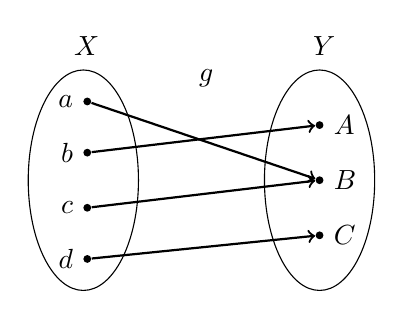
\begin{tikzpicture}
			\draw \boundellipse{0,0}{0.7}{1.4};
			\draw \boundellipse{3,0}{0.7}{1.4};
			\node[circle,fill,inner sep=1pt] (a) at (0.05,1.0) [label=left:$a$]{};
			\node[circle,fill,inner sep=1pt] (b) at (0.05,0.35) [label=left:$b$]{};
			\node[circle,fill,inner sep=1pt] (c) at (0.05,-0.35) [label=left:$c$]{};
			\node[circle,fill,inner sep=1pt] (d) at (0.05,-1.0) [label=left:$d$]{}; 
			\node[] at (0.45,1.7) [label=left:$X$]{}; 
			\node[circle,fill,inner sep=1pt] (A) at (3.0,0.7) [label=right:$A$]{};
			\node[circle,fill,inner sep=1pt] (B) at (3.0,0.0) [label=right:$B$]{};
			\node[circle,fill,inner sep=1pt] (C) at (3.0,-0.7) [label=right:$C$]{}; 
			\node[] at (3.45,1.7) [label=left:$Y$]{}; 
			\node[] at (1.9,1.3) [label=left:$g$]{}; 
			\draw[->,thick] (a) to (B);
			\draw[->,thick] (b) to (A);
			\draw[->,thick] (c) to (B);
			\draw[->,thick] (d) to(C);
			\end{tikzpicture}
			\caption{En funktion $g$.}
			\label{fig:fun11}
		\end{minipage}
		\begin{minipage}{0.49\textwidth}
			\centering
			\pgfplotsset{width=0.5\textwidth,compat=1.11}
			\centering
			\begin{tikzpicture}
						\draw \boundellipse{0,0}{0.7}{1.4};
			\draw \boundellipse{3,0}{0.7}{1.4};
			\node[circle,fill,inner sep=1pt] at (0.05,1.0) [label=left:$a$]{};
			\node[circle,fill,inner sep=1pt] at (0.05,0.35) [label=left:$b$]{};
			\node[circle,fill,inner sep=1pt] at (0.05,-0.35) [label=left:$c$]{};
			\node[circle,fill,inner sep=1pt] at (0.05,-1.0) [label=left:$d$]{}; 
			\node[] at (0.45,1.7) [label=left:$X$]{}; 
			\node[circle,fill,inner sep=1pt] at (3.0,0.7) [label=right:$A$]{};
			\node[circle,fill,inner sep=1pt] at (3.0,0.0) [label=right:$B$]{};
			\node[circle,fill,inner sep=1pt] at (3.0,-0.7) [label=right:$C$]{}; 
			\node[] at (3.45,1.7) [label=left:$Y$]{}; 
			\node[] at (1.9,1.3) [label=left:$f$]{}; 
			\draw[->,thick] (a) to (A);
			\draw[->,thick] (b) to (A);
			\draw[->,thick] (c) to (C);
			\draw[->,thick] (d) to (C);
			\end{tikzpicture}
			\caption{En funktion $f$.}
			\label{fig:fun1}
		\end{minipage}
	\end{figure}
\end{frame}
\section{Sammensatte funktioner}
\begin{frame}{Funktioner}{Sammensatte funktioner}
\begin{itemize}
		\setlength\itemsep{1em}
	\item<1-> Hvis $f\colon X\to Y$ og $g\colon Y\to Z$ så kan vi definere sammensætningen $g\circ f\colon X\to Z$ ved $(g\circ f)(x)=g(f(x))$.
	\item<8-> Funktionen $f$ kaldes den \emph{indre funktion} og $g$ kaldes den \emph{ydre funktion}.
%	\item Figur~\ref{fig:fun2} viser en skitse af funktionssammensætning.
	\item<9-> Eksempel: Sammensæt $f(x)=\sqrt{x}$ med $g(x)=e^{2x}$.\setbeamercovered{} \onslide<10->{ Svar: $(f\circ g)(x)=\sqrt{e^{2x}}=e^x$,} \onslide<11->{$ (g\circ f)(x)=e^{2\sqrt{x}} $}
\end{itemize}

	\begin{figure}[!htbp]
		\pgfplotsset{width=0.5\textwidth,compat=1.11}
		\centering
		\resizebox{8.0cm}{!}{%
		\begin{tikzpicture}
		\draw[visible on = <2->] \boundellipse{0,0}{0.7}{1.4};
		\draw[visible on = <3->] \boundellipse{5,0}{0.7}{1.4};
		\draw[visible on = <5->] \boundellipse{10,0}{0.7}{1.4};
		\node[visible on = <2->] at (0.45,1.7) [label=left:\only<2->{$X$}]{};
		\node[visible on = <3->] at (5.45,1.7) [label=left:\only<3->{$Y$}]{}; 
		\node[visible on = <5->] at (10.45,1.7) [label=left:\only<5->{$Z$}]{}; 
		\node[circle, fill,inner sep=1pt,visible on = <4->] (x) at (0.05,0) [label=left:\only<4->{$x$}]{};
		\node[circle, fill,inner sep=1pt, visible on = <4->] (fx) at (5.05,0) [label=left:\only<4->{$f(x)$}]{};
		\node[circle, fill,inner sep=1pt, visible on = <6->] (gfx) at (10.05,0) [label=left:\only<6->{$g(f(x))$}]{};
		\draw[thick,->,visible on=<4->] (x) to [bend right] node[pos=0.5, label=above:$f$] {} (fx) ;
		\draw[thick,->,visible on=<6->] (fx) to [bend right] node[pos=0.5, label=above:$g$] {} (gfx) ;
		\draw[thick,->,visible on=<7->] (x) to [bend left] node[pos=0.5, label=below:$g\circ f$] {} (gfx) ;
		\end{tikzpicture}%
	}%
%		\caption{En sammensat funktion.}
%		\label{fig:fun2}
	\end{figure}%
\end{frame}

\begin{frame}{Funktioner}{Første-og andengradspolynomier}
\begin{itemize}
		\setlength\itemsep{1em}
	\item<1-> Et førstegradspolynomium er en funktion med forskrift på formen
	\begin{align*}
	f(x)=ax+b.
	\end{align*}
	\item<2-> Grafen for et førstegradspolynomium er en ret linje med hældning $a$ som skærer $y$-aksen i $b$.
	\item<3-> Et andengradspolynomium er en funktion med forskrift på formen
	\begin{align*}
	f(x)=ax^2+bx+c.
	\end{align*}
	\item<4-> Grafen for et andengradspolynomium er en parabel som skærer $y$-aksen i $c$.
	
\end{itemize}
\end{frame}
\section{Første-og andengradspolynomier}
\begin{frame}{Funktioner}{Første-og andengradspolynomier}
\begin{itemize}
	\item<1-> Figur~\ref{fig:fun3} Viser eksempler på første-og andengradspolynomier.
\end{itemize}
\begin{figure}
			\centering
		\resizebox{5.0cm}{!}{%
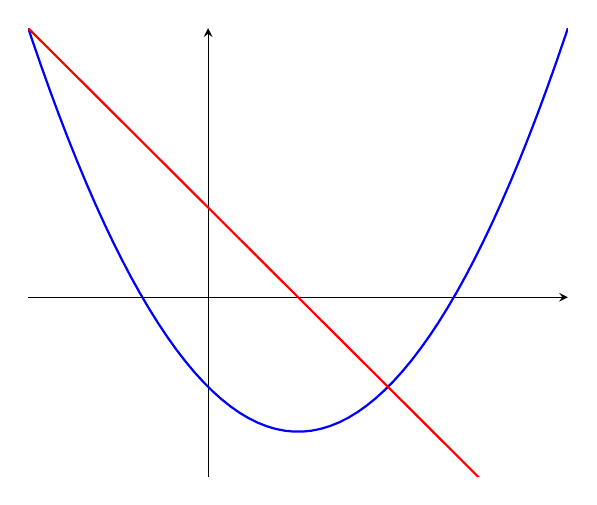
\begin{tikzpicture}
\begin{axis}[xmin=-1,xmax=2,ymin=-2,ymax=3,axis x line=center,
axis y line=center,ticks=none]
\addplot[thick,blue,samples=200]{2*x^2-2*x-1};
\addplot[thick,red,samples=200] {-2*x+1};
\end{axis}
\end{tikzpicture}%
}%
\caption{Grafer for første-og andengradspolynomier.}
\label{fig:fun3}
\end{figure}
\end{frame}


\section{Inverse funktioner}
\begin{frame}{Inverse funktioner}
\begin{itemize}
		\setlength\itemsep{1em}
	\item To funktioner $f\colon X\to Y$ og $g\colon Y\to X$ er hinandens \emph{inverse} hvis
	\begin{align*}
	f(g(y))=y,\quad \textup{og}\quad g(f(x))=x 
	\end{align*}
	 for alle $x$ i $X$ og $y$ i $Y$.
	 \item<9-> Eksempel: $f(x)=x^2$ og $g(x)=\sqrt{x}$ begge defineret på $[0,\infty[$ er inverse funktioner.
	 \item<10-> Eksempel: $f(x)=\frac{1}{x}$ defineret på $\R\setminus\{0\}$ er sin egen invers.
	 
	 %\item I Figur~\ref{fig:fun4} er to inverse funktioner skitseret.
\end{itemize}
	 \begin{figure}[!htbp]
	\pgfplotsset{width=0.5\textwidth,compat=1.11}
	\centering
	\resizebox{5cm}{!}{%
		\begin{tikzpicture}
		\draw[visible on=<2->] \boundellipse{0,0}{0.7}{1.4};
		\draw[visible on=<2->] \boundellipse{5,0}{0.7}{1.4};
		\node[visible on=<2->] at (0.45,1.7) [label=left:\only<2->{$X$}]{};
		\node[visible on=<2->] at (5.45,1.7) [label=left:\only<2->{$Y$}]{}; 
		\node[circle,fill,inner sep=1pt,visible on=<3->] (x) at (0,1) [label=below:\only<3->{$x$}] {};
		\node[circle,fill,inner sep=1pt,visible on=<7->] (gy) at (0,-1) [label=above:\only<7->{$g(y)$}] {};
		\node[circle,fill,inner sep=1pt,visible on=<4->] (fx) at (5,1) [label=below:\only<4->{$f(x)$}] {};
		\node[circle,fill,inner sep=1pt,visible on=<6->] (y) at (5,-1) [label=above:\only<6->{$y$}] {};
		\draw[thick,->,visible on=<4->] (x) to[bend left]node[pos =0.5, label=below: \only<4->{$f$}] {} (fx);
		\draw[thick,->,visible on=<5->] (fx) to[bend left] node[pos =0.5, label=above:\only<5->{$g$}] {} (x);
		\draw[thick,->,visible on=<7->] (y) to[bend left]node[pos =0.5, label=above: \only<7->{$g$}] {} (gy);
		\draw[thick,->,visible on =<8->] (gy) to[bend left]node[pos =0.5, label=below: \only<8->{$f$}] {} (y);
		\end{tikzpicture}%
	}%
%	\caption{Inverse funktioner.}	 
%	\label{fig:fun4}%
\end{figure}
\end{frame}

\section{Logaritmer og eksponentialfunktioner}
\begin{frame}{Logaritmer og eksponentialfunktioner}
\begin{itemize}
			\setlength\itemsep{1em}
	\item<1-> For ethvert positivt $a\neq 1$ kalder vi funktionen $f_a\colon \R\to ]0,\infty[$ givet ved $f_a(x)=a^x$ for \emph{eksponentialfunktionen med grundtal $a$}.
	\item<2-> Funktionen $f_a(x)=a^x$ har en invers funktion $\log_a\colon ]0,\infty[\to \R$ som kaldes \emph{logaritmen med grundtal $a$}.
	\item<3-> Hvis $a=e$ så skriver vi $\ln$ i stedet for $\log_e$ og hvis $a=10$ skriver vi $\log$ i stedet for $\log_{10}$.
	\item<4-> Der gælder at
	\begin{align*}
	log_a(a^x)=x\quad \textup{og} \quad a^{\log_a(y)}=y,
	\end{align*}
	for alle $x\in \R$ og $y\in ]0,\infty[$.
	\item<5-> Eksempler: Udregn
\end{itemize}
	\begin{align*}
\onslide<5->{\log_2(8),}&&\onslide<6->{\log_{10}(10000),}&&\onslide<7->{\log_a(1).}
\end{align*}
\end{frame}

\begin{frame}{Logaritmer og eksponentialfunktioner}{Regneregler}
\begin{itemize}
			\setlength\itemsep{1em}
	\item<1-> Når vi arbejder med eksponentialfunktioner kan vi anvende potensregneregler.
	\item<2-> For logaritmer har vi følgende regneregler
	\end{itemize}
	\begin{align*}
	\onslide<2->{\log_a(xy)&=\log_a(x)+\log_a(y),}\\\onslide<3->{\log_a(\frac{x}{y})&=\log_a(x)-\log_a(y),}\\ \onslide<4->{
	\log_a(x^r)&=r\log_a(x).}%,&&\log_a(x)=\frac{\ln(x)}{\ln(a)}.
	\end{align*}
	\begin{itemize}
	\item<5-> Eksempler: Udregn
\end{itemize}
\begin{align*}
\onslide<5->{\log(50)+\log(20),}&& \onslide<6->{2^{2+\log_2(5)},}&& \onslide<7->{9^{\log_3(2)}.}
\end{align*}
\end{frame}

\section{Trigonometriske funktioner}
\begin{frame}{Trigonometriske funktioner}
\begin{itemize}
	\item<1-> Vi definerer de trigonometriske funktioner ud fra enhedscirklen.
\end{itemize}
\begin{figure}
	\centering
	\resizebox{5cm}{!}{%
		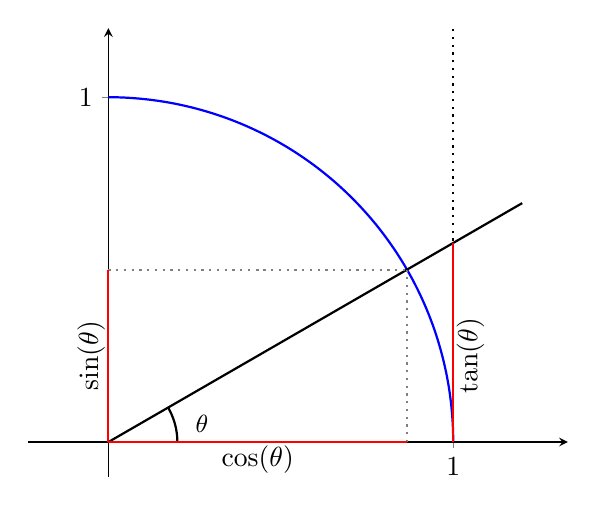
\begin{tikzpicture}
		\begin{axis}[xmin=-0.1,xmax=1.2,ymin=-0.1,ymax=1.2,axis x line=center,
		axis y line=center, axis equal, xtick={0,1},ytick={0,1}]
		%PERMANENT STUFF
		\addplot[blue,domain=0:pi/2,thick, samples=100] ({cos(deg(x))},{sin(deg(x))});
		\addplot[domain=0:sqrt(3)/2,thick] {1/sqrt(3)*x};
		\addplot[domain=0:pi/6,thick,samples=100] ({0.2*cos(deg(x))},{0.2*sin(deg(x))}) node[label=right:{\small$\theta$},pos=0.5] {};
		%SHOW THIS FIRST
		\addplot[dotted,gray,thick,visible on=<2->] coordinates {(sqrt(3)/2,0) (sqrt(3)/2, 1/2)};
		\node[visible on=<3->] at (axis cs: {sqrt(3)/4},-0.05) {$\cos(\theta)$};
		\addplot[thick,red,domain=0:sqrt(3)/2,visible on=<3-4>] {0};
		%SHOW THIS SECOND
		%\node[visible on=<3->,label={[label distance=0cm,text depth=-1ex,rotate=90]:$\sin(\theta)$}] at (axis cs:-0.1,1/4) {};
		\node[visible on=<5->] at (axis cs: -0.05,1/4) {\rotatebox{90}{$\sin(\theta)$}};
		\addplot[dotted, gray,thick,domain=0:sqrt(3)/2,visible on=<4->] {1/2};	
		\addplot[thick,red,visible on=<5-6>]  coordinates { (0,0) (0,1/2)};
		%SHOW THIS THIRD
		\addplot[thick,domain=sqrt(3)/2:1.2,visible on= <6->] {1/sqrt(3)*x};
		\addplot[thick,dotted,visible on=<6->] coordinates {(1,0) (1,1.2)};
		%\node[label={[label distance=0cm,text depth=-1ex,rotate=90]:$\tan(\theta)$},visible on=<4->] at (axis cs:1.1,1/4) {};
		\node[visible on=<7->] at (axis cs: 1.05,1/4) {\rotatebox{90}{$\tan(\theta)$}};
		\addplot[red,thick,visible on=<7->] coordinates {(1,0) (1, 1/sqrt(3)};

		\end{axis}
		\end{tikzpicture}%
	}%
\end{figure}
\begin{itemize}
	\item<8-> Bemærk at $\tan(\theta)=\frac{\sin(\theta)}{\cos(\theta)}$.
\end{itemize}
\end{frame}

\begin{frame}{Trigonometriske funktioner}{Eksakte værdier}
\begin{itemize}
	\item For særlige vinkler kan vi bestemme eksakte værdier af de trigonometriske funktioner.
\end{itemize}
\begin{minipage}{0.49\textwidth}
\resizebox{5cm}{!}{%	
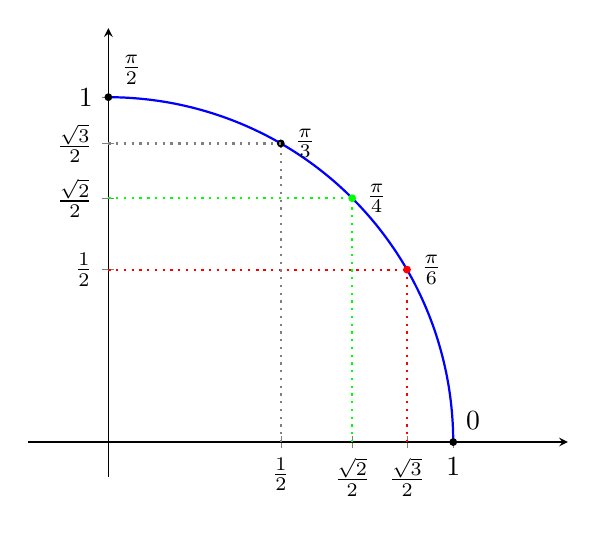
\begin{tikzpicture}
\begin{axis}[xmin=-0.1,xmax=1.2,ymin=-0.1,ymax=1.2,axis x line=center,
axis y line=center, axis equal, xtick={0,1/2,sqrt(2)/2,sqrt(3)/2,1},ytick={0,1/2,sqrt(2)/2,sqrt(3)/2,1}, xticklabels={$0$, $\frac{1}{2}$,$\frac{\sqrt{2}}{2}$,$\frac{\sqrt{3}}{2}$,$1$}, yticklabels={$0$, $\frac{1}{2}$,$\frac{\sqrt{2}}{2}$,$\frac{\sqrt{3}}{2}$,$1$}]
%PERMANENT STUFF
\addplot[blue,domain=0:pi/2,thick, samples=100] ({cos(deg(x))},{sin(deg(x))});
\node[circle,fill,inner sep=1pt,label=above right:$0$] at (axis cs: 1,0) {};
\node[circle,fill,inner sep=1pt,label=above right:$\frac{\pi}{2}$] at (axis cs: 0,1) {};
%PI/6
\addplot[dotted,thick,visible on =<3->,red] coordinates {(sqrt(3)/2,0) (sqrt(3)/2, 1/2)};
\node[circle,fill,inner sep=1pt,label=right:$\frac{\pi}{6}$,red] at (axis cs: {sqrt(3)/2},1/2) {};
\addplot[dotted,thick,domain=0:sqrt(3)/2,visible on =<3->,red] {1/2};	
%PI/4
\addplot[dotted,thick,visible on =<4->,green] coordinates {(sqrt(2)/2,0) ({sqrt(2)/2}, {sqrt(2)/2})};
\node[circle,fill,inner sep=1pt,label=right:$\frac{\pi}{4}$,green] at (axis cs: {sqrt(2)/2},{sqrt(2)/2}) {};
\addplot[dotted,thick,domain=0:sqrt(2)/2,visible on =<4->,green] {sqrt(2)/2};	
%PI/3
\addplot[dotted,gray,thick,visible on =<5->] coordinates {(1/2,0) (1/2,{sqrt(3)/2})};
\node[circle,fill,inner sep=1pt,label=right:$\frac{\pi}{3}$] at (axis cs: 1/2,{sqrt(3)/2}) {};
\addplot[dotted, gray,thick,domain=0:1/2,visible on =<5->] {sqrt(3)/2};
\end{axis}
\end{tikzpicture}%
}%
\end{minipage}
\begin{minipage}{0.49\textwidth}
\begin{table}[h!]
	\begin{tabular}{@{} lccc @{}}
	\toprule 
		$\theta$			& $\sin \theta$			& $\cos \theta$ 		& $\tan \theta$ 		\\ \midrule
		0					\onslide<2->{&0						&1						&0			}\\
		$ \frac{\pi}{6} $	\onslide<3->{&$\frac{1}{2}$			&$\frac{\sqrt{3}}{2}$	&$\frac{1}{\sqrt{3}}$}	\\
		$ \frac{\pi}{4} $	\onslide<4->{&$\frac{\sqrt{2}}{2}$	&$\frac{\sqrt{2}}{2}$	&$1$				}	\\
		$ \frac{\pi}{3} $	\onslide<5->{&$\frac{\sqrt{3}}{2}$	&$\frac{1}{2}$			&$\sqrt{3}$			}	\\
		$ \frac{\pi}{2} $	\onslide<6->{&1						&0						&					}	\\
		\bottomrule  
	\end{tabular}
\end{table}
\end{minipage}
\end{frame}

\begin{frame}{Trigonometriske funktioner}{Eksempler}
\begin{itemize}
			\setlength\itemsep{1em}
	\item<1-> Når I skal løse opgaver så tegn altid enhedscirklen og udnyt symmetri.
	\item<2-> Eksempler: Udregn
\end{itemize}
\begin{align*}
\onslide<2->{\cos(\frac{2\pi}{3}),}&& \onslide<6->{\sin(9\pi),}&& \onslide<7->{\sin(-\frac{5\pi}{4}).}
\end{align*}
\onslide<2->{%
\begin{figure}
	\resizebox{4.5cm}{!}{%	
		\begin{tikzpicture}
		\begin{axis}[xmin=-1.1,xmax=1.1,ymin=-1.1,ymax=1.1,axis x line=center,
		axis y line=center, axis equal, xtick={-1,1},ytick={-1,1}, xticklabels={$-1$,$1$}, yticklabels={$-1$,$1$}]
		%PERMANENT STUFF
		\addplot[blue,domain=0:2*pi,thick, samples=100] ({cos(deg(x))},{sin(deg(x))});
%		%FIRST
		\node[circle,fill,inner sep=1pt,label=right:\only<3-5>{$\frac{\pi}{3}$}, visible on=<3-5>] at (axis cs: 1/2,{sqrt(3)/2}) {};
		\node[circle,fill,inner sep=1pt,label=left:\only<4-5>{$\frac{2\pi}{3}$},visible on=<4-5>] at (axis cs: -1/2,{sqrt(3)/2}) {};
		\addplot[dotted,gray,thick,visible on =<5-5>] coordinates {(1/2,0) (1/2,{sqrt(3)/2})};
		\addplot[dotted,gray,thick,visible on =<5-5>] coordinates {(-1/2,0) (-1/2,{sqrt(3)/2})};

		\node[circle,fill,inner sep=1pt,label=above left:\only<{6,10-}>{$\pi$},visible on={<6,10->}] at (axis cs: -1,0) {};		

		
		\node[circle,fill,inner sep=1pt,label=left:\only<11->{$-\frac{5\pi}{4}$},visible on=<11->] at (axis cs: {-sqrt(2)/2},{sqrt(2)/2}) {};
		\node[circle,fill,inner sep=1pt,label=right:\only<7->{$-\frac{\pi}{4}$},visible on=<7->] at (axis cs: {sqrt(2)/2},{-sqrt(2)/2}) {};
		\node[circle,fill,inner sep=1pt,label=right:\only<7->{$\frac{\pi}{4}$},visible on=<7->] at (axis cs: {sqrt(2)/2},{sqrt(2)/2}) {};
		\node[circle,fill,inner sep=1pt,label=above:\only<8->{$-\frac{\pi}{2}$},visible on=<8->] at (axis cs: 0,-1) {};		
		\node[circle,fill,inner sep=1pt,label=left:\only<9->{$-\frac{3\pi}{4}$},visible on=<9->] at (axis cs: {-sqrt(2)/2},{-sqrt(2)/2}) {};		
		\addplot[dotted,gray,thick,visible on =<12>,domain=-sqrt(2)/2:sqrt(2)/2]  {sqrt(2)/2};

		
		


		
%		\addplot[dotted, gray,thick,domain=0:1/2,visible on =<5->] {sqrt(3)/2};
%
%		%PI/4
%		\addplot[dotted,thick,visible on =<4->,green] coordinates {(sqrt(2)/2,0) ({sqrt(2)/2}, {sqrt(2)/2})};
%		\node[circle,fill,inner sep=1pt,label=right:$\frac{\pi}{4}$,green] at (axis cs: {sqrt(2)/2},{sqrt(2)/2}) {};
%		\addplot[dotted,thick,domain=0:sqrt(2)/2,visible on =<4->,green] {sqrt(2)/2};	
%		%PI/3

		\end{axis}
		\end{tikzpicture}%
	}%
\end{figure}%
}
\end{frame}














%\section{Differentialregning}
\begin{frame}{Differentialregning}
\begin{itemize}
	\item<1-> Differentialregning omhandler bestemmelse af hældninger af funktioner.
	\item<2-> Vi definerer en funktions hældning vha. sekanter.
\end{itemize}
\begin{figure}
	\resizebox{5cm}{!}{%	
		\begin{tikzpicture}
		\begin{axis}[xmin=-2.1,xmax=2.3,ymin=-0.5,ymax=2.7,axis x line=center,
		axis y line=center, axis equal,ticks=none]
		\addplot[thick,blue,samples=300] {ln(x+2)/ln(2)+1/2};
		\node[circle,fill,inner sep=1pt,label=above left:\only<{3-}>{$(x_0,f(x_0)$)},visible on={<3->}] at (axis cs: -1,1/2) {};		
		\node[circle,fill,inner sep=1pt,label=below:\only<{3-}>{$ x_0 $},visible on={<3->}] at (axis cs: -1,0) {};
		
		\node[circle,fill,inner sep=1pt,label=below:\only<{4-4}>{$ x_0+3 $},visible on={<4-4>}] at (axis cs: 2,0) {};
		\node[circle,fill,inner sep=1pt,visible on =<4->] at (axis cs: 2,5/2) {};
		\addplot[thick,black,visible on=<4-4>] {2*x/3+7/6};
		
		
	\node[circle,fill,inner sep=1pt,label=below:\only<{5}>{$ x_0+1 $},visible on={<5>}] at (axis cs: 0,0) {};
	\node[circle,fill,inner sep=1pt,visible on =<5->] at (axis cs: 0,3/2) {};
	\addplot[thick,black,visible on=<5>] {x+3/2};
	\addplot[thick,gray,dashed,visible on=<5->] {2*x/3+7/6};
	
	\node[circle,fill,inner sep=1pt,label=below:\only<{6}>{$ x_0+\frac{1}{2}$},visible on={<6>}] at (axis cs: -1/2,0) {};
	\node[circle,fill,inner sep=1pt,visible on =<6>] at (axis cs: -1/2,{ln(3/2)/ln(2)+1/2}) {};
	\addplot[thick,black,visible on=<6>] {2*ln(3/2)/ln(2)*x+ln(81/8)/ln(4)};
	\addplot[thick,gray,dashed,visible on=<6->] {x+3/2};
	

	\addplot[thick,gray,dashed,visible on=<7->] {2*ln(3/2)/ln(2)*x+ln(81/8)/ln(4)};
	\addplot[thick,red,visible on =<7->] {1/ln(2)*(x+1)+1/2};
	
		\end{axis}
		\end{tikzpicture}%
	}%
\end{figure}
\end{frame}

\begin{frame}{Differentialregning}
\begin{itemize}
			\setlength\itemsep{1em}
	\item<1-> En funktion $f$ er differentiabel i $x_0$ hvis grænsen
	\begin{align*}
	f'(x_0)=\lim_{h\to 0}\frac{f(x_0+h)-f(x_0)}{h}
	\end{align*}
	eksisterer.
	\item<2-> Bemærk at $f'(x)$ betegner hældningen af $f$ i $x$.
	\item<3-> Vi anvender ofte notationen
	\begin{align*}
	f'(x)=\frac{d}{dx} f(x)=\frac{df}{dx}(x).
	\end{align*}
\end{itemize}
\end{frame}

\section{Regneregler for kendte funktioner}
\begin{frame}{Differentialregning}{Regneregler}
\begin{itemize}
			\setlength\itemsep{1em}
	\item<1-> Vi har følgende regneregler:
\end{itemize}
\begin{minipage}{0.49\textwidth}
	\centering
	\begin{tabular}{@{}l c@{}}
\onslide<1->{$f(x)$      & $f'(x)$}  				\\ \toprule
\onslide<2->{$c$			& $0$} 					\\ \midrule
\onslide<3->{$x$			& $1$}					\\ \midrule
\onslide<4->{$x^n$  		& $nx^{n-1}$}			\\ \midrule
\onslide<5->{$e^x$  		& $e^x$}					\\ \midrule
\onslide<6->{$e^{cx}$  	& $ce^{cx}$}				\\ \bottomrule
	\end{tabular}
\end{minipage}
\begin{minipage}{0.49\textwidth}
	\centering
\begin{tabular}{@{}l c@{}}
\onslide<1->{$f(x)$      & $f'(x)$}  				\\ \toprule
\onslide<7->{$a^x$  		& $a^x\ln a $}			\\ \midrule
\onslide<8->{$\ln x$ 	& $\frac{1}{x}$}			\\ \midrule
\onslide<9->{$\cos x$  	& $-\sin x$}				\\ \midrule
\onslide<10->{$\sin x$  	& $\cos x$}				\\ \midrule
\onslide<11->{$\tan x$ 	& $1+\tan^2(x)$}		\\ \bottomrule  
\end{tabular}
\end{minipage}
\begin{itemize}
			\setlength\itemsep{1em}
	\item<12-> Eksempler: Differentier funktionerne 
\end{itemize}
\begin{align*}
\onslide<12->{f(x)=\sqrt{x},}&& \onslide<13->{g(x)=\frac{1}{x},}&& \onslide<14->{h(x)=\ln(x^3).}
\end{align*}
\end{frame}
\section{Generelle regneregler}
\begin{frame}{Differentialregning}{Regneregler}
\begin{itemize}
			\setlength\itemsep{1em}
	\item<1-> Vi har følgende generelle regneregler
	\end{itemize}
	\begin{align*}
	\onslide<1->{(cf)'(x)&=cf'(x)}\\
	\onslide<2->{(f\pm g)'(x)&=f'(x)\pm g'(x).}
	\end{align*}
	\begin{itemize}
	\item<3-> Eksempler: Differentier funktionerne 
\end{itemize}
\begin{align*}
\onslide<3->{f(x)=2x+1-\frac{1}{x},}&& \onslide<4->{ g(x)=3x^{-2}-2e^{-x}+\cos(x)}
\end{align*}
\end{frame}

%\section{Repetition af regneregler}
\begin{frame}{Differentialregning}{Repetition af regneregler}
\begin{itemize}
	\setlength\itemsep{1em}
	\item Vi har følgende regneregler:
\end{itemize}
\begin{minipage}{0.49\textwidth}
	\centering
	\begin{tabular}{@{}l c@{}}
		$f(x)$      & $f'(x)$  				\\ \toprule
		$c$			& $0$ 					\\ \midrule
		$x$			& $1$					\\ \midrule
		$x^n$  		& $nx^{n-1}$			\\ \midrule
		$e^x$  		& $e^x$					\\ \midrule
		$e^{cx}$  	& $ce^{cx}$				\\ \bottomrule
	\end{tabular}
\end{minipage}
\begin{minipage}{0.49\textwidth}
	\centering
	\begin{tabular}{@{}l c@{}}
		$f(x)$      & $f'(x)$  				\\ \toprule
		$a^x$  		& $a^x\ln a $			\\ \midrule
		$\ln x$ 	& $\frac{1}{x}$			\\ \midrule
		$\cos x$  	& $-\sin x$				\\ \midrule
		$\sin x$  	& $\cos x$				\\ \midrule
		$\tan x$ 	& $1+\tan^2(x)$		\\ \bottomrule  
	\end{tabular}
\end{minipage}
\vspace{1em}
\begin{itemize}
	\setlength\itemsep{1em}
	\item<2-> Samt $(cf)'(x)=cf'(x)$ og $(f\pm g)'(x)=f'(x)\pm g'(x)$.
\end{itemize}
\end{frame}

\section{Produkt-og kvotientientreglen}
\begin{frame}{Produkt-og kvotientientreglen}
\begin{itemize}
				\setlength\itemsep{1em}
	\item<1-> For produkter og kvotienter af funktioner har vi følgende regneregler
	\end{itemize}
	\begin{align*}
	\onslide<1->{(fg)'(x)&=f'(x)g(x)+f(x)g'(x)}\\
	\onslide<2->{\Big(\frac{f}{g}\Big)'(x)&=\frac{f'(x)g(x)-f(x)g'(x)}{g^2(x)}}
	\end{align*}
	\begin{itemize}
	\item<3-> Eksempler: Differentier funktionerne
\end{itemize}
\begin{align*}
\onslide<3->{f(x)=xe^{2x},}&&\onslide<4->{g(x)=\frac{\cos(x)}{x},}&& \onslide<5->{h(x)=\cos(x)\sin(x).}
\end{align*}
\end{frame}


\section{Kædereglen}
\begin{frame}{Kædereglen}
\begin{itemize}
				\setlength\itemsep{1em}
	\item<1-> Husk at sammensatte funktioner er på formen 
	\begin{align*}
	(f\circ g)(x)=f(g(x)).
	\end{align*}
	\item<2-> Sammensatte funktioner differentieres med kædereglen:
	\begin{align*}
	(f\circ g)'(x)=f'(g(x))g'(x).
	\end{align*}
	\item<3-> Eksempler: Differentier funktionerne 
\end{itemize}
	\begin{align*}
	\onslide<3->{f(x)=\cos(x^2),}&& \onslide<4->{g(x)=e^{x^3+3x},}&&\onslide<5->{h(x)=\sin^2(x^2-2x+1)}
	\end{align*}
	\begin{itemize}
	\item<6-> Eksempel: Differentier funktionen $f(x)=xe^{\sqrt{x}}$.
\end{itemize}
\end{frame}
%\section{Ubestemte integraler}
\begin{frame}{Ubestemte integraler}{Stamfunktioner}
\begin{itemize}
	\setlength\itemsep{1em}
	\item<1-> En funktion $f$ har stamfunktion $F$ hvis
	\begin{align*}
	F'(x)=f(x)
	\end{align*}
	\item<2-> Hvis $F$ er stamfunktion til $f$ så er $F(x)+c$ også, for alle $c\in \R$.
	\item<3-> Det ubestemte integral af $f$ defineres til
	\begin{align*}
	\int f(x)\, dx =F(x)+c,
	\end{align*}
	hvor $F$ er en stamfunktion til $f$ og $c\in \R$.
	\item<4-> Eksempler: Er $e^{x^2}$ stamfunktion til $2xe^{x^2}$?
\end{itemize}
\end{frame}

\section{Regneregler for ubestemte integraler}
\begin{frame}{Regneregler for ubestemte integraler}
\begin{itemize}
	\setlength\itemsep{1em}
	\item<1-> Vi har følgende regneregler:
\end{itemize}
\begin{minipage}{0.49\textwidth}
	\centering
	\begin{tabular}{@{}l c@{}}
\onslide<1->{$f(x)$      & $\int f(x)\, dx$}  		\\ \toprule
\onslide<2->{$c$			& $cx+k$} 				\\ \midrule
\onslide<3->{$x$			& $\frac{1}{2}x^2+k$}	\\ \midrule
\onslide<4->{$x^n$  		& $\frac{1}{n+1}x^{n+1}+k$, $(n\neq -1)$}	\\ \midrule
\onslide<5->{$e^x$  		& $e^x+k$}					\\ \midrule
\onslide<6->{$e^{cx}$  	& $\frac{1}{c}e^{cx}+k$}				\\ \bottomrule
	\end{tabular}
\end{minipage}
\begin{minipage}{0.49\textwidth}
	\centering
	\begin{tabular}{@{}l c@{}}
\onslide<1->{$f(x)$      & $\int f(x)\, dx$}  				\\ \toprule
\onslide<7->{$\frac{1}{x}$ & $\ln(\vert x\vert)+k $}			\\ \midrule
\onslide<8->{$\ln x$ 	& $x\ln(x)-x+k$}			\\ \midrule
\onslide<9->{$\cos x$  	& $\sin x+k$}				\\ \midrule
\onslide<10->{$\sin x$  	& $-\cos x+k$}				\\ \midrule
\onslide<11->{$\tan x$ 	& $-\ln(\vert \cos(x)\vert)+k$}		\\ \bottomrule  
	\end{tabular}
\end{minipage}
\vspace{1em}
\begin{itemize}
	\item<12-> Eksempler:   
\end{itemize}
\vspace{-0.5cm}
\begin{align*}
\onslide<12->{\int \sqrt{x}\,d x,}&&\onslide<13->{\int x^3\, d x}
\end{align*}
\end{frame}

\begin{frame}{Regneregler for ubestemte integraler}
\begin{itemize}
		\setlength\itemsep{1em}
	\item<1-> Vi har følgende generelle regneregler
	\begin{align*}
	\onslide<1->{\int cf(x) \, d x&=c\int f(x)\, dx}\\
	\onslide<2->{\int f(x)\pm g(x) \, d x&=\int f(x)\, dx\pm \int g(x) \, dx.}
	\end{align*}
	\item<3-> Eksempler: Udregn
\end{itemize}
	\begin{align*}
\onslide<3->{\int e^{3x}+\sqrt[3]{x}+1\, dx,}\\
\onslide<4->{\int \frac{1}{2x}-cos(x)\, dx.}
\end{align*}
\end{frame}

\section{Bestemte integraler}
\begin{frame}{Bestemte integraler}
\begin{itemize}
		\setlength\itemsep{1em}
	\item<1-> Vi vil bestemme arealer under grafer for funktioner.
	\item<2-> Arealet mellem grafen for $f$ og $x$-asksen i intervallet $[a,b]$ er givet ved
	\begin{align*}
	F(b)-F(a),
	\end{align*} 
	hvor $F$ er en stamfunktion til $f$.
	\item<3-> Derfor defineres det bestemte integral af $f$ i intervallet $[a,b]$ til
	\begin{align*}
	\int_a^b f(x)\, dx =[F(x)]_a^b=F(b)-F(a).
	\end{align*}
	\item<4-> Eksempel: Bestem $\int_0^1 x^2 \, d x$.
\end{itemize}
\end{frame}

\section{Regneregler for bestemte integraler}
\begin{frame}{Regneregler for bestemte integraler}

\begin{itemize}
\setlength\itemsep{1em}
 \item<1-> Vi har følgende generelle regneregler for bestemte integraler
 	\begin{align*}
 \onslide<1->{\int_a^b cf(x) \, d x&=c\int_a^b f(x)\, dx}\\
 \onslide<2->{\int_a^b f(x)\pm g(x) \, d x&=\int_a^b f(x)\, dx\pm \int_a^b g(x) \, dx.}
 %\int_a^b f(x)\, dx&=\int_a^c f(x) \, dx+\int_c^b f(x) \, dx\\
 %\int_a^b f(x)\, dx&=-\int_b^a f(x) \, dx.
 \end{align*}
 \item<3-> Eksempler: Udregn
\end{itemize}
 \begin{align*}
\onslide<3->{\int_1^2 \frac{1}{2x}-1 \, dx}\\
\onslide<4->{\int_0^4 3x^2+3e^x \, dx.}
\end{align*}
\end{frame}



%\section{Delvis integration}
\begin{frame}{Delvis integration}
\begin{itemize}
	\setlength\itemsep{1em}
	\item<1-> Skal man integrere produkter af funktioner anvendes delvis integration:
\end{itemize}
	\begin{align*}
	\onslide<1->{\int f(x)g(x)\, dx&=f(x)G(x)-\int f'(x)G(x)\, dx}\\
	\onslide<2->{\int_a^b f(x)g(x)\, dx&=[f(x)G(x)]_a^b-\int_a^b f'(x)G(x)\, dx}
	\end{align*}
	\begin{itemize}
	\item<3-> Det er ikke lige meget hvordan $f$ og $g$ vælges.
	\item<4-> Eksempler: Udregn
\end{itemize}
	\begin{align*}
\onslide<4->{\int xe^x \, dx,\setbeamercovered{}\onslide<5->{&\setbeamercovered{}=xe^x-\int e^x \, dx}\onslide<6->{=xe^x-e^x}}\\
\onslide<7->{\int_0^{\frac{\pi}{2}} x\sin (x)\, dx\setbeamercovered{}\onslide<8->{&\setbeamercovered{}=[x(-\cos(x))]_0^\frac{\pi}{2}-\int_0^\frac{\pi}{2}(-\cos(x))\, dx\onslide<9->{=\int_0^\frac{\pi}{2} \cos(x)\, dx\onslide<10->{=[\sin(x)]_0^\frac{\pi}{2}\onslide<11->{=1}}}}.}
\end{align*}
\end{frame}

\section{Integration ved substitution}
\begin{frame}{Integration ved substitution}
\begin{itemize}
		\setlength\itemsep{1em}
	\item<1-> For integration af sammensatte funktioner gælder at
\end{itemize}
	\begin{align*}
	\onslide<1->{\int f(g(x))g'(x)\, dx &=F(g(x))+c}\\
	\onslide<2->{\int_a^b f(g(x))g'(x) \, dx&=[F(g(x))]_{a}^{b}.}
	\end{align*}
	\begin{itemize}
	\item<3-> Denne regneregel kaldes integration ved substitution.
	\item<4-> Vi vil ofte anvende en særlig metode der retfærdiggør navnet.
\end{itemize}
\end{frame}

\begin{frame}{Integration ved substitution}{Ubestemt integral}
\begin{minipage}{0.45\textwidth}
	\begin{itemize}
		\setlength\itemsep{1em}
		\item<1-> Udregn $\int f(g(x))g'(x)\, dx$.
		\item<2-> Lad $u=g(x)$.
		\item<3-> Udregn $\frac{du}{dx}$ og isoler $dx$.
		\item<4-> Substituer $g(x)$ og $dx$.
		\item<5-> Udregn integralet mht. $u$.
		\item<6-> Substituer tilbage.
	\end{itemize}
\end{minipage}
\onslide<7->{%
\begin{minipage}{0.54\textwidth}
	\begin{itemize}
				\setlength\itemsep{1em}
		\item<7-> Udregn $\int x^2\cos(x^3)\, dx$.
		\item<8-> Lad $u=x^3$.
		\item<9-> Så er $\frac{du}{dx}=3x^2$ og $dx=\frac{du}{3x^2}$.
		\item<10-> $\int x^2\cos(u)\frac{du}{3x^2}\, du=\frac{1}{3}\int \cos(u)\, du$
		\item<11-> $\frac{1}{3}\int \cos(u)\, du=\frac{1}{3}\sin(u)+c$.
		\item<12-> $\int x^2\cos(x^3)\, dx=\frac{1}{3}\sin(x^3)+c$.
	\end{itemize}
\end{minipage}%
}
\end{frame}

\begin{frame}{Integration ved substitution}{Bestemt integral}
\begin{minipage}{0.47\textwidth}
	
	\begin{itemize}
		\setlength\itemsep{1em}
		\item<1-> Udregn $\int_a^b f(g(x))g'(x)\, dx$.
		\item<2-> Lad $u=g(x)$.
		\item<3-> Udregn $\frac{du}{dx}$ og isoler $dx$.
		\item<4-> Substituer $g(x)$, $dx$ samt grænser.
		\item<5-> Udregn integralet mht. $u$.
	\end{itemize}
\end{minipage}
\onslide<6->{%}
\begin{minipage}{0.52\textwidth}
	\begin{itemize}
		\setlength\itemsep{1em}
		\item<6-> Udregn $\int_{-1}^2 -xe^{x^2}\, dx$.
		\item<7-> Lad $u=x^2$.
		\item<8-> Så er $\frac{du}{dx}=2x$ og $dx=\frac{du}{2x}$.
		\item<9-> $\int_{1}^4 -xe^{u}\, \frac{du}{2x}=-\frac{1}{2}\int_1^4 e^u\, du$
		\item<10-> $\frac{-1}{2}\int_1^4 e^u\, du=\frac{-1}{2}[e^u]_1^4=\frac{e-e^4}{2}$.
	\end{itemize}
\end{minipage}%
}
\end{frame}




{\aauwavesbg
\begin{frame}[plain,noframenumbering]
  \finalpage{Opgaveregning!}
\end{frame}}
%%%%%%%%%%%%%%%%

\end{document}
